\subsection{Component Identification in Figure T-1}
\label{T6C05}

\begin{tcolorbox}[colback=gray!10!white,colframe=black!75!black,title=T6C05]
What is component 4 in figure T-1?

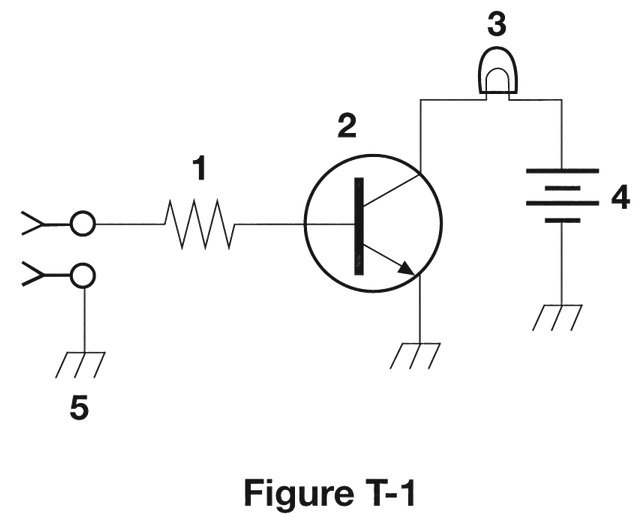
\includegraphics[width=0.5\textwidth]{tech/images/t1.png} 



\begin{enumerate}[label=\Alph*)]
    \item Resistor
    \item Transistor
    \item Ground symbol
    \item \textbf{Battery}
\end{enumerate}
\end{tcolorbox}

\subsubsection{Intuitive Explanation}
Imagine you're looking at a treasure map, and you need to figure out what the fourth symbol on the map represents. In this case, the map is Figure T-1, and the symbol is component 4. Just like a treasure map has symbols for trees, rivers, and treasure chests, Figure T-1 has symbols for different electronic parts. The correct answer is the battery, which is like the energy source that powers everything, just like the sun powers a solar-powered toy.

\subsubsection{Advanced Explanation}
In electronic schematics, components are represented by standardized symbols. Figure T-1 is a schematic diagram that includes various components labeled with numbers. Component 4 is identified by its symbol, which corresponds to a battery. A battery in a schematic is typically represented by a series of alternating long and short lines, indicating the positive and negative terminals. 

The battery is a crucial component in any electronic circuit as it provides the necessary voltage to power the circuit. The voltage (V) supplied by the battery can be calculated using Ohm's Law, which states that \( V = I \times R \), where \( I \) is the current and \( R \) is the resistance in the circuit. Understanding the role and representation of each component in a schematic is fundamental for analyzing and designing electronic circuits.

% Prompt for generating the diagram: Create a schematic diagram labeled Figure T-1 with various components, clearly marking component 4 as a battery.